%% ============================================================
%%  Chapter 1 - Cloud Computing: Foundations and Security
%%  All citations verified with real DOIs (IEEE Access, NIST, MDPI)
%% ============================================================

\chapter{Cloud Computing: Foundations and Security}
\label{chap:cloud}

\section{Introduction}
\label{sec:cloud_intro}

Cloud computing is not a technology by itself, rather it is a delivery model. The underlying technologies (e.g. Virtualization, network storage, distributed computing) already exist for a long time before cloud computing was an established term. What occurred in or around 2006 is a change in business model, it was the month of August in 2006 when Amazon released its Elastic Compute Cloud (EC2) which provides compute instances, or bare metal computing power, as a commodity service available on demand for a small fee based on an hourly rate\cite{aws_ec2_announcement2006}. The transition from owning a piece of hardware to renting an available computing instance became the hallmark feature of cloud computing, and it changed the way every company works today.
Understanding the basics of the cloud delivery model is key to the context of this project as the nature of the security attacks it has to identify cannot be generically stated as attacks over the network, rather they must be addressed within the constraints of a cloud environment. Concepts like multi-tenancy, resource pooling, elasticity, API-driven interfaces make a cloud system susceptible to specific attack vectors for which perimeter security appliances were not built.
This chapter will elaborate on the features and delivery models of cloud computing and cloud deployment options along with the associated security threats.

% ─────────────────────────────────────────────────────────────
\section{Definition and Essential Characteristics}
\label{sec:cloud_def}

The definition that is quoted most often within the literature, both academic and industrial, is by the US National Institute of Standards and Technology. Mell and Grance state that cloud computing is "\textit{a model for enabling ubiquitous, convenient, on-demand network access to a shared pool of configurable computing resources [\ldots] that can be rapidly provisioned and released with minimal management effort or service provider interaction}" \cite{mell2011nist}. This definition has endured well as it is based on the visible behavior and not on specific technologies (e.g. The hypervisor or networking stack).

NIST recognizes 5 inherent characteristics which we will consider along with the security implications for each:

\begin{enumerate}[label=\alph*.]

  \item \textbf{On-demand self-service:} A user can independently provision resources,via a portal or via API, without the intervention of a support representative for the provider.While it is operationally appealing to provision quickly, a compromised account can launch hundreds of VMs within minutes-whether to do cryptomining or use the VMs as a base for attacks.

  \item \textbf{Broad network access:} Cloud resources are accessed through regular network protocols on any device. Each instance with a public IP address is always exposed to internet-scale scanning and brute force attacks.

  \item \textbf{Resource pooling:} Through virtualisation, a single set of physical hardware is shared among tenants at the same time. Data from one tenant sits on a physical machine alongside the workload of another tenant, separated only by software boundaries. When those software boundaries break down (due to hypervisor vulnerabilities or side-channel attacks), so does the assurance of isolation.

  \item \textbf{Rapid elasticity:} Scaling automatically occurs, both up and down.
From a monitoring point of view, this has as a consequence that the set of machines to be monitored is never stable. New endpoints are constantly being created and destroyed, and monitoring on IP addresses alone would fail.

  \item \textbf{Measured service:} All resources consumed are accounted for and measured.
This is, in fact, a security benefit, cloud computing provides the logs of API call history, network flows, storage access etc. Which form the basis of intrusion detection.

\end{enumerate}

% ─────────────────────────────────────────────────────────────
\section{Cloud Service Models}
\label{sec:service_models}

IaaS, PaaS, SaaS are three different service models to identify how much of the stack is to be managed by the service provider and how much is the responsibility of the consumer. From there it is determined that which aspects can be monitored and what aspects can be configured by the customer, and subsequently which are to be protected from threat.

\subsection{Infrastructure as a Service}

With IaaS, the service provider offers virtualised compute, storage and networking. The client, on the other hand, has control over all the layers above the hypervisor: the OS, middleware, applications, and data. Examples of IaaS include AWS EC2, Google Compute Engine, and Azure Virtual Machines.
IaaS offers the greatest control to the client, but also the greatest responsibility. The customer is responsible for configuring which ports they expose, which services to run, how to configure the firewalls etc. A rule to an incorrectly configured security group, such as opening SSH access to everyone on the internet, is fully the customer's responsibility to fix; the provider has only gone as far as the hypervisor layer \cite{nist2011architecture}. This is the correct model to use for this project, the lab itself is comprised of two virtual machines run on a KVM hypervisor, and the types of attacks experimented with are just the types of attack faced by customers on services exposed via IaaS.

\subsection{Platform as a Service}

\ac{PaaS} also abstracts the customer out from under the operating system, the cloud provider offers runtime and middleware and lets the customer push up applications. That is how products such as Google App Engine and Heroku operate. The customer cannot install a network inspection agent or record raw packet flow;visibility in the infrastructure level is lost. That restricts what a standard NIDS will observe, and shifts the threat focus to application-level vulnerabilities like application layer injection and authentication bypassing attacks.

\subsection{Software as a Service}

\ac{SaaS} provides a complete application, e.g.Microsoft 365 or Salesforce. Provider is responsible for maintaining the application, the customer is responsible for managing user accounts, data sharing, and access policies. There is no role for a network intrusion detection device such as project. The security control here will be identity and access management, and data loss prevention.

\subsection{Shared responsibility boundary}

At the core of organising the security responsibilities for all 3 cloud models is the \textit{shared responsibility model}: responsibility is distributed between cloud provider who is responsible for what’s below the border, and the user is responsible for anything above the border \cite{nist2011architecture}. Table~\ref{tab:shared_responsibility} depicts what that border changes to in each of the models.

\begin{table}[H]
  \centering
  \caption{Security responsibility distribution(P = Provider, C = Customer)}
  \label{tab:shared_responsibility}
  \renewcommand{\arraystretch}{1.4}
  \begin{tabularx}{\textwidth}{lXXX}
    \toprule
    \textbf{Stack layer} & \textbf{IaaS} & \textbf{PaaS} & \textbf{SaaS} \\
    \midrule
    Physical infrastructure & P & P & P \\
    Network fabric \& hypervisor & P & P & P \\
    Operating system & C & P & P \\
    Middleware \& runtime & C & P & P \\
    Application & C & C & P \\
    Data \& access control & C & C & C \\
    \bottomrule
  \end{tabularx}
\end{table}

Looking at the table it’s clear IaaS is where a customer has the most in the way of security responsibilities. Four out of six tiers are customer owned and owned means that network intrusion detection is in play.

% ─────────────────────────────────────────────────────────────
\section{Cloud Deployment Models}
\label{sec:deployment_models}

The service model defines what's being delivered, the deployment model define who gets to consume the service and who runs the service. The four deployment models has different security perspectives on the service provided.

\subsection{Public cloud}

Resources are owned and managed by a provider and accessible by multiple over the Internet. This involves several organizations running applications, data and software on the same hardware (in this process also referred to as ‘multi- tenancy’), whether it is public clouds like AWS, Azure and GCP, provider owns the data center space, security as well as managing hypervisor. Customer receives elasticity and economies of scales by surrendering management control of some of the physical.

\subsection{Private cloud}

You are given infrastructure exclusively for the use of one organization. It can reside in your own data center or in your colocation facility; it doesn’t contain the infrastructure of multiple tenants. The most popular open-source platform for building a private cloud is OpenStack. 
Banks, healthcare organizations, the military and defense have their own private clouds because their data, or the law, requires keeping it in one location. 
This cloud scenario is relevant to this project because the organization which has own the private cloud doesn’t have access to cloud services like AWS GuardDuty, Azure Defender etc. That tools can run only within the environment they were created from. This company must implement its own detection mechanisms; the current system can exactly address this requirement.

\subsection{Hybrid cloud}

A hybrid cloud means pairing a company’s internal, private IT infrastructure with at least one external public cloud provider. Less-sensitive or scalable workload in the public cloud, while a firm can run high-priority, security-sensitive applications internally. Communications flow across this environment via a VPN connection or a dedicated, secure network line. When considering a hybrid approach, there are new challenges in thinking about a defined boundary: the environments have different levels of inherent trust, and security can’t be applied on a hop-by-hop basis.

% ─────────────────────────────────────────────────────────────
\section{Cloud Architecture Essentials}
\label{sec:cloud_arch}

There are two approaches to cloud architectural design which are significant enough to need short explanations in the context of security virtualization, and the network model used within cloud architecture.

\subsection{Virtualisation and the hypervisor}
 Virtualization is enabling a single piece of hardware to run several separate, simultaneous instances of an operating system. A hypervisor acts as the layer between the physical hardware and the guest OSes, and isolates them each by providing them with the same hardware profile view.

Type-1 hypervisors (bare-metal) exist directly on top of hardware: Examples include Xen, or VMware ESXi. Type-2 hypervisors exist as a process within the context of a host OS, and they expose the underlying hardware from within the guest to multiple guests. KVM can be thought of as a bit of a hybrid between the two: It is a Linux kernel module, effectively transforming the Linux kernel itself into a Type-1 hypervisor. It is very commonly deployed with private clouds, and KVM is the hypervisor found running in our lab.

The hypervisor is the primary security boundary for the cloud. If an exploit that allows one guest operating system to read another guest's memory is possible -- also known as a VM escape -- it pretty much negates everything. Those are extremely rare, but they do happen -- as for example the 2015 VENOM flaw (CVE-2015-3456), a guest-to-host escape due to a buggy virtual floppy drive implementation in QEMU\cite{crowdstrike_venom2015}. Thus hypervisor updates are as urgently prioritized as the patching of kernels in production clouds.
\subsection{Network model: virtual networks and east-west traffic}

Within a cloud the network traffic is performed by a software layer that replaces the functionality of a physical switch and router. Customers define “virtual networks” called virtual private clouds (VPCs) at AWS which include own addressing schemes, address ranges, subnets, etc.. Within a virtual network virtual machines don’t send out and receive packets by hardware which has not stayed on the local physical host the vm lives on, traffic stays entirely on software the virtual switch on the host(s). 
The security relevant aspect is the traffic classification: there are “north-south” and “east-west” network connections. 
North-south traffic is connection that starts and end out side of the cloud provider cloud infrastructure and passes its border and so traditionally would pass a “perimeter” firewall. East-west traffic moves within cloud provider infrastructure, e.g. From service A in VM B to service C in VM D and vice versa, these traffic volumes currently account for the largest part of network traffic in cloud data centers and can be on same host (see Figure~\ref{fig:cloud_traffic}). Those east-west traffic volumes never had to leave the perimeter to arrive at its destination \cite{kfoury2024smartnics}, thus they went by mostly uninspected. 
A network-based IDS placed within the virtual network, inspecting also east-west traffic, is required to cover this blind-spot.

\begin{figure}[H]
  \centering
  \IfFileExists{figures/cloud_traffic_directions.png}{%
    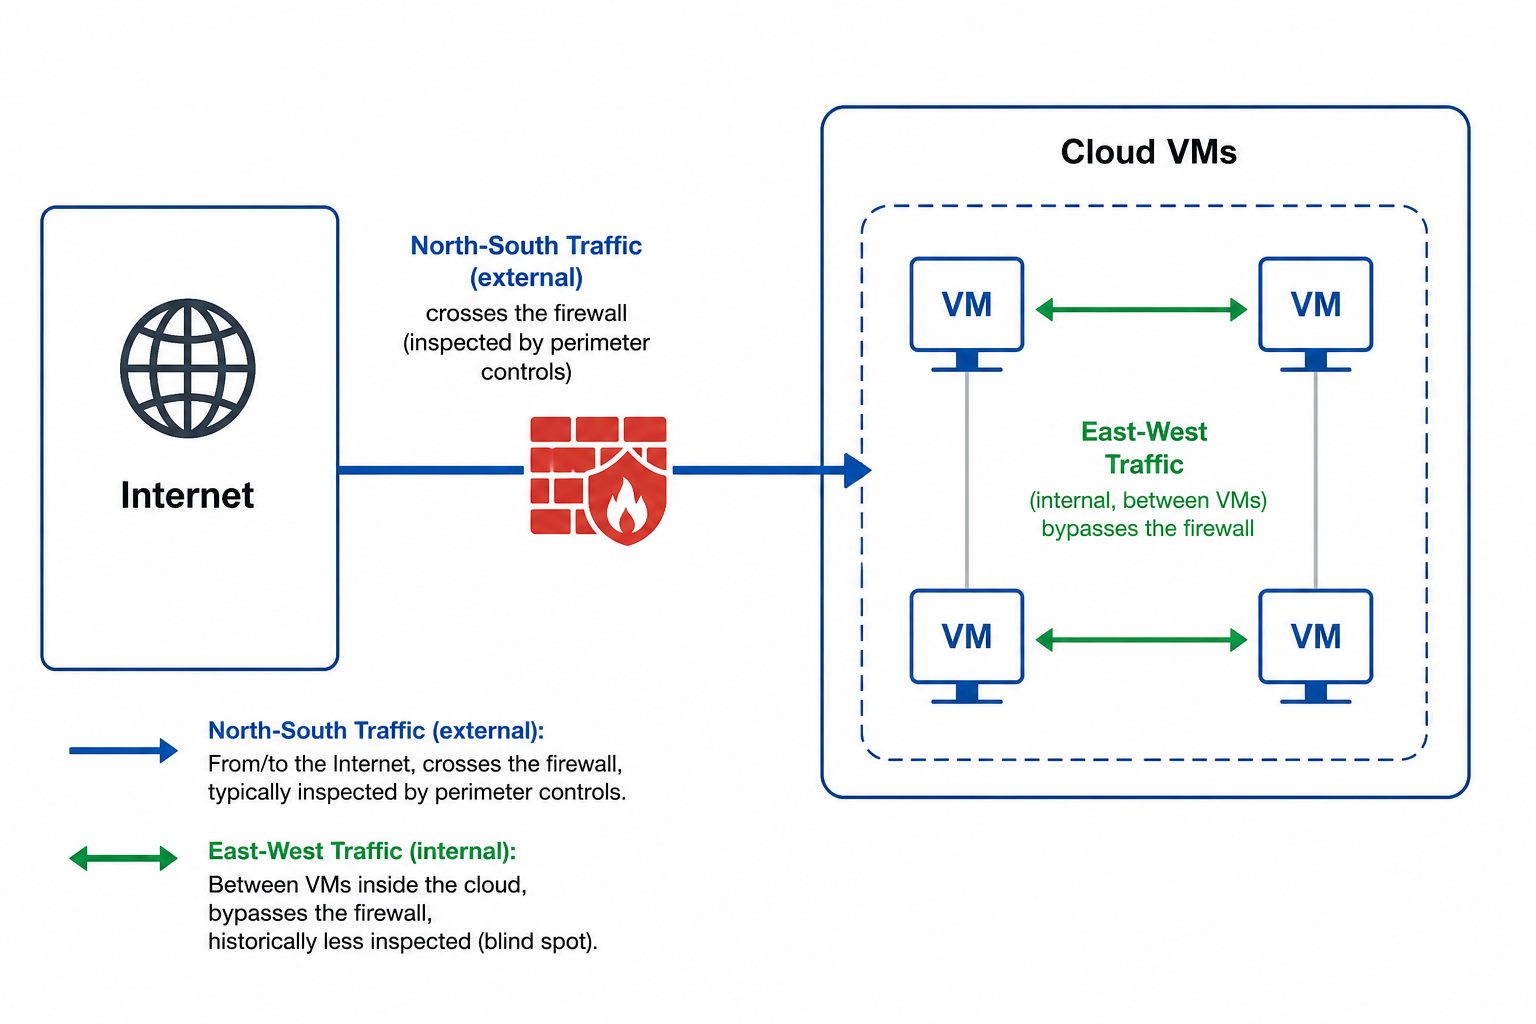
\includegraphics[width=0.82\textwidth]{figures/cloud_traffic_directions.png}%
  }{%
    \fbox{\parbox{0.75\textwidth}{\centering\vspace{1.2cm}
    \texttt{[Figure: cloud\_traffic\_directions.png, to be created]}\\[4pt]
    \small This is a simple original diagram (two boxes: ``Internet'' and
    ``Cloud VMs'', with a labelled arrow for north-south traffic crossing a
    firewall icon, and a separate labelled arrow for east-west traffic between
    VMs that bypasses the firewall). No external image needed, draw directly
    in PowerPoint, draw.io, or a tikzpicture.
    \vspace{1.2cm}}}%
  }
  \caption{North-south vs\ east-west traffic in a cloud environment}
  \label{fig:cloud_traffic}
\end{figure}


% Source for figure: draw it yourself or adapt from the NIST architecture diagrams
% at https://nvlpubs.nist.gov/nistpubs/Legacy/SP/nistspecialpublication500-292.pdf
% (NIST SP 500-292, open access, no copyright restrictions)

% ─────────────────────────────────────────────────────────────
\section{Security Challenges in Cloud Environments}
\label{sec:cloud_security}

The same qualities that make operationally attractive the cloud shared, scalable remote and API also represent the cause of its most severe security pitfalls. A systematic survey done by Alouffi et al. \cite{alouffi2021systematic} in the body of 80 reviewed articles about the safety of cloud found seven predominant classes of risks, with data leaking and manipulation and Unauthorized accessing occurring most often in those research articles surveyed. Next few subsections detail four kinds of risks primarily of network level intrusion detection significance.

\subsection{Misconfiguration}
It’s universally agreed that a significant portion of cloud security breaches is due to misconfiguration, the low-hanging fruit of open storage buckets, a too-generous firewall ruleset or disabled logging, all readily identified by automated scanners within minutes of their deployment. Cloud threat reports have also regularly listedmisconfigured services,insecure interfaces and weak access control as recurring vulnerability categories plaguing cloud users \cite{tabrizchi2020survey}.

The issue with misconfiguration is the effect of scale; if one IAM policy applied to 100 different instances and someone misconfigures it and all 100 will inherit the misconfiguration instantly. In a legacy environment, on prem misconfiguration could impact one or few servers but in the cloud, an individual misconfiguration could impact your entire data asset.

For IDS misconfiguration provides opportunity for compensating controls even the root issue is misconfiguration, IDS logs are able to capture the exploit of the misconfiguration once the hacker decides to exploit it, when hacker will scan a new exposed port or brute force against service that should never be exposed.

\subsection{Brute-force attacks on exposed services}

Any service that exposes itself externally to the internet over a network interface is susceptible to an automated credential attack against its exposed endpoint for example, port SSH (22), port RDP (3389), port database (5432), or port on an application web UI login page. In the cloud, every instance with a public IP address will be subjected to constant, automated attacks within minutes of it appearing on the public internet. 

Nadeem et al. Show that cloud networks are under perpetual attacks with constant automated brute force and DDoS attack attempts, and that IDS systems successfully interrupt many attacks when configured well \cite{nadeem2021intercept}. 

Brute force attacks result in a unique signature in terms of the volume of connection attempts targeting port Y on some destination device that originates from the same, or a small set of source IPs, with a higher ratio of attempted than completed successful connections. These signatures are readily detectable using flow level statistics, the primary features contained in the CICIDS2017 data set used in this investigation.

\subsection{Denial-of-service attacks}

DDos attack seeks to saturate server's resource bandwidth, CPU, connection table to make its unusable. Cloud elasticity protects against volumetric attack of DDos through bursting. A cloud can scale out the service and can accommodate high rate. But this service is limited, an excessive amount of volumetric attack will result in a great increase in service usage and consequently costs will go up due to the increase in the bandwidth usage.

The low rate application layer attacks, like RUDY, Slow loris, hold on to the established TCP connections with a small amount of data by a slowly increasing number of connections and are much harder to be detected. By holding the TCP connection to the server open with a small quantity of data, the attackers can successfully exhaust a server's resource and connection tables. Agrawal and Tapaswi in their research demonstrated that low-rate application-layer denial of service (DDoS) attacks (e.g. RUDY and Slowloris) have traffic characteristics close to normal slow clients, thus, difficult to detect through rate thresholds \cite{agrawal2019ddos}. 
Detection would probably require statistical approach and evaluation on the time windows.

\subsection{Lateral movement}

When a system is compromised, it by exploiting a vulnerable service, stealing credentials, or executing a phishing payload-an intruder will often perform lateral movement: exploring nearby systems within the network, also a virtual network, in an effort to increase their attack surface and gain access to additional resources or sensitive data. Since traffic that moves east to west generally avoids perimeter controls and analysis, the intruders' movement within an organization may go unnoticed for days or weeks. The MITRE ATT\&CK knowledge base, in its matrix dedicated to cloud environments, catalogues lateral movement as one of the core tactics of a cloud intrusion; the techniques it lists under this tactic include the reuse of stolen credentials and authentication material across services and the abuse of legitimate remote-management channels, usually preceded by internal discovery activity such as scanning for reachable services \cite{mitre_attack_cloud}. As internal traffic must be monitored for lateral movement attacks, internal visibility must be integrated into the design of any IDS.
Table~\ref{tab:cloud_threats} summarises the four threat categories and their key
detectable signatures.

\begin{table}[H]
  \centering
  \caption{Threats in cloud environments and their detection
           signatures in flow data.}
  \label{tab:cloud_threats}
  \renewcommand{\arraystretch}{1.4}
  \begin{tabularx}{\textwidth}{lXX}
    \toprule
    \textbf{Threat} & \textbf{Mechanism} & \textbf{Flow-level signature} \\
    \midrule
    Misconfiguration exploitation
      & Attacker targets an unintentionally exposed service
      & Rapid sequential port connections; unusual source geography \\
    \midrule
    Brute force
      & Automated credential guessing against SSH/RDP/HTTP
      & High connection count to single port; high failure rate; short sessions \\
    \midrule
    DDoS
      & Traffic flood (volumetric) or connection exhaustion (low-rate)
      & Abnormal packet rate or count; SYN flag anomalies; long session durations \\
    \midrule
    Lateral movement
      & Internal network probing and service exploitation after initial compromise
      & Unusual east-west flows; sequential internal port scans; new \\
        service-to-service communication patterns \\
    \bottomrule
  \end{tabularx}
\end{table}

% ─────────────────────────────────────────────────────────────
\section{Why Standard Security Tools Fall Short}
\label{sec:cloud_tools_limits}

The challenge with security appliances was that they were built around an era of networks with clear boundaries. A hardware firewall sits at the perimeter, an on-prem IDS sniffs the traffic going across the core switch. Neither idea translate to the cloud quite so neatly. 
In the cloud firewalls are really just named access control lists attached to each individual VM  security groups, not some centrally managed piece of hardware. 
And if your traffic between VM’s on the same host never makes it’s way across the physical network hardware, it won’t get seen by traditional network taps. While commercial cloud offerings from AWS GuardDuty and Microsoft Defender for Cloud address some of this, they only offer protection in a specific, proprietary cloud and they provide no access to the underlying logic. 
Running a private cloud on OpenStack or KVM ?
Good luck finding default detection tools there. 
It is precisely this gap which prompts the creation of an open and deployable ML based system to identify anomalous behavior across clouds using off the shelf components.

% ─────────────────────────────────────────────────────────────
\section{Summary}
\label{sec:cloud_summary}

Cloud computing itself is characteristically described by five qualities which are particularly security relevant; on-demand self-service makes it very easy for attackers to escalate quickly, widespread network access constantly offers a large attack surface for exposed services, resource pooling allows attackers to risk the security of other cloud occupants, elasticity makes constant static monitoring obsolete, and measured service makes useful logs available for event detection. As the infrastructure as a service, where the client is responsible for everything in the stack above the hypervisor, can impose the largest risk on security, we treat the Iaas as the most important service. In particular for Private and hybrid clouds, there’s a need for stand-alone detection tools, because the commercial “Cloud-Native” detection solutions don’t operate in these clouds. 

Three major attacks at the network level; brute-forcing, DDoS, and lateral movement, leave distinctive signatures on flow level, these signatures form our target in the detection system presented in this report and are present in the training and evaluation dataset. 
Chapter two: will provide a brief introduction of machine learning algorithms used for automatic recognition of those signatures.
